%!TEX root = ../thesis.tex
%*******************************************************************************
%*********************************** First Chapter *****************************
%*******************************************************************************

\chapter{Boundary Condition Consistency}  %Title of the First Chapter

\ifpdf
    \graphicspath{{Chapter10/Figs/Raster/}{Chapter10/Figs/PDF/}{Chapter10/Figs/}}
\else
    \graphicspath{{Chapter10/Figs/Vector/}{Chapter10/Figs/}}
\fi

\label{chapter 10}


%************************************************************************** 

The perfect conducting wall condition is validated in the rotated Brio-Wu test in chapter \ref{chapter 4}, with reflective Dirichlet $B_n$ and transmissive Neumann $B_t$. The resistive boundary condition represented by equation \ref{equ:magneticDiffusion} is applied in cylindrical equilibrium in chapter \ref{chapter 8}, with a whole copy for $\mathbf{B}$ from wall to plasma ghost cells, similar to most of resistive wall relevant studies \cite{chrysanthou2020,ferraro2016multi,becerra2016resistive,hender1989effects}. These boundary condition approaches have been commonly used for modeling perfect conducting walls and resistive walls. Yet, it seems that when the resistivity approaches zero, the resistive condition is still quite different from when the resistivity is exactly zero. Even the resistive wall model based on equation \ref{equ:magneticDiffusion} in Chapter \ref{chapter 7} does not have an agreement with the perfect conducting mathematical model we established in Chapter \ref{chapter 2}. This results in significantly different numerical conditions depending on whether $\eta_{w}>0$, as discussed in the previous chapter. This is further visualized in Figure \ref{fig:totalEnergy}, where the total energy curves gap between $\eta_w=0.0$ and $\eta_w=0.001$ is quite large. In this chapter, we are going to analyze superconducting wall condition and extend these into a general wall condition, which may help to address this inconsistency.

\section{Superconducting Wall Condition}
\subsection{London Equations}
The London Equations provide some magnetic distributions in superconductors. It starts from the definition of current density. As in around page 147 of Kittle \cite{kittel2018introduction}, the current density is defined as  
$$
\mathbf{J}_s=-n_s q_e \mathbf{v}_s\ ,
$$
Where the $q_e$ is the elementary charge on a single electron with  $q_e=-1.602176634\times10^{-19}$, a negative number. The $n_s$ and $\mathbf{v}_s$, in simple terms, are electron number density and velocity, where lower index $s$ specify a superconductor situation. We have the Newton's Second Law of Motion for electron \cite{kittel2018introduction} 
\begin{equation}
m\frac{d\mathbf{v}_s}{dt}=-q_e\mathbf{E}\ ,
\label{equ:motion_perfectConducting}
\end{equation}
where $m$ is the electron mass and $\mathbf{E}$ is the electric field. For these basic laws and the Meissner effect on superconductor, the first and second London Equation are proposed
$$
\frac{\partial \mathbf{J}_s}{\partial t}=\frac{n_s q_e^2}{m}\mathbf{E}\ ,
$$
$$
\frac{\partial }{\partial t}\left(\nabla\times\mathbf{J}_s+\frac{n_s q_e^2}{m}\mathbf{B}\right)=0\ \Rightarrow\ 
\nabla\times\mathbf{J}_s+\frac{n_s q_e^2}{m}\mathbf{B}=0\ .
$$
A further conclusion is given  
\begin{equation}
	\nabla^2\mathbf{B}=\frac{1}{\lambda_s^2}\mathbf{B}\ ,\ \ \ \ \ \  \lambda_s^2=\frac{m}{n_s q_e^2}\ .
	\label{equ:B_superconducting}
\end{equation}


\subsection{Penetration on Superconductor Wall}
This equation \ref{equ:B_superconducting} gives us some information on the magnetic field within superconductors. If we place a magnetic field, we may know about the strength distribution and how the superconducting wall reflect the normal component of magnetic field. We place a wall in a vacuum. As depicted in Plot \ref{fig:magneticPenetration}, a normal magnetic $\mathbf{B}=B_0\mathbf{i}$ is suddenly imposed on the wall, with the x-direction being the only significant one. This results in an equation that applies along the x-axis.
\begin{equation}
	\frac{\partial^2 B_x}{\partial x^2}=\frac{1}{\lambda_s^2}B_x\ .
\end{equation}
It is a homogeneous second order differential equation, a Helmholtz equation. Some physical boundary conditions are given as $B_x(0)=B_0$ and $\lim_{x \to \infty} B_x(x)=0$. These define the solution
\begin{equation*}
	B_x(x)=B_0e^{-\frac{x}{\lambda_s}}\ .
\end{equation*}
$\lambda_s$ is "penetration depth" controlling the penetration. Even for superconductors, there will be some penetration. As discussed in chapter \ref{chapter 6}, the superconducting materials used in ITER and EAST are Nb3Sn and NbTi. Their penetration depths are around $\lambda_{Nb3Sn}=8.0\times10^{-8}m$ and $\lambda_{NbTi}=1.0\times10^{-7}m$. The free electron density of various metals is of the same order of magnitude around $10^{28}$. Therefore, the difference in $\lambda$ should be within one or two orders of magnitude. However, for a better visualization, we add a simple nonphysical case    $\lambda_{0}=4.6\times10^{-4}m$ showing the penetration curve on plots. Their penetrations under simply $B_0=1.0$ are demonstrated in Figure \ref{fig:PenetrationCurveSuperconducting}. The x-axis is scaled to the 0.001 level because similar subdivision lengths are typically used in the simulation's mesh refinement. In the plot, once the magnetic field penetrate into a superconducting wall, it is fully countered off. This form a 'no-penetration' condition on superconducting for normal component. A reflective boundary condition is applied under this scenario. We have proved these mathematically in chapter \ref{chapter 2}. 
 
\begin{figure}[H]
	\centering
	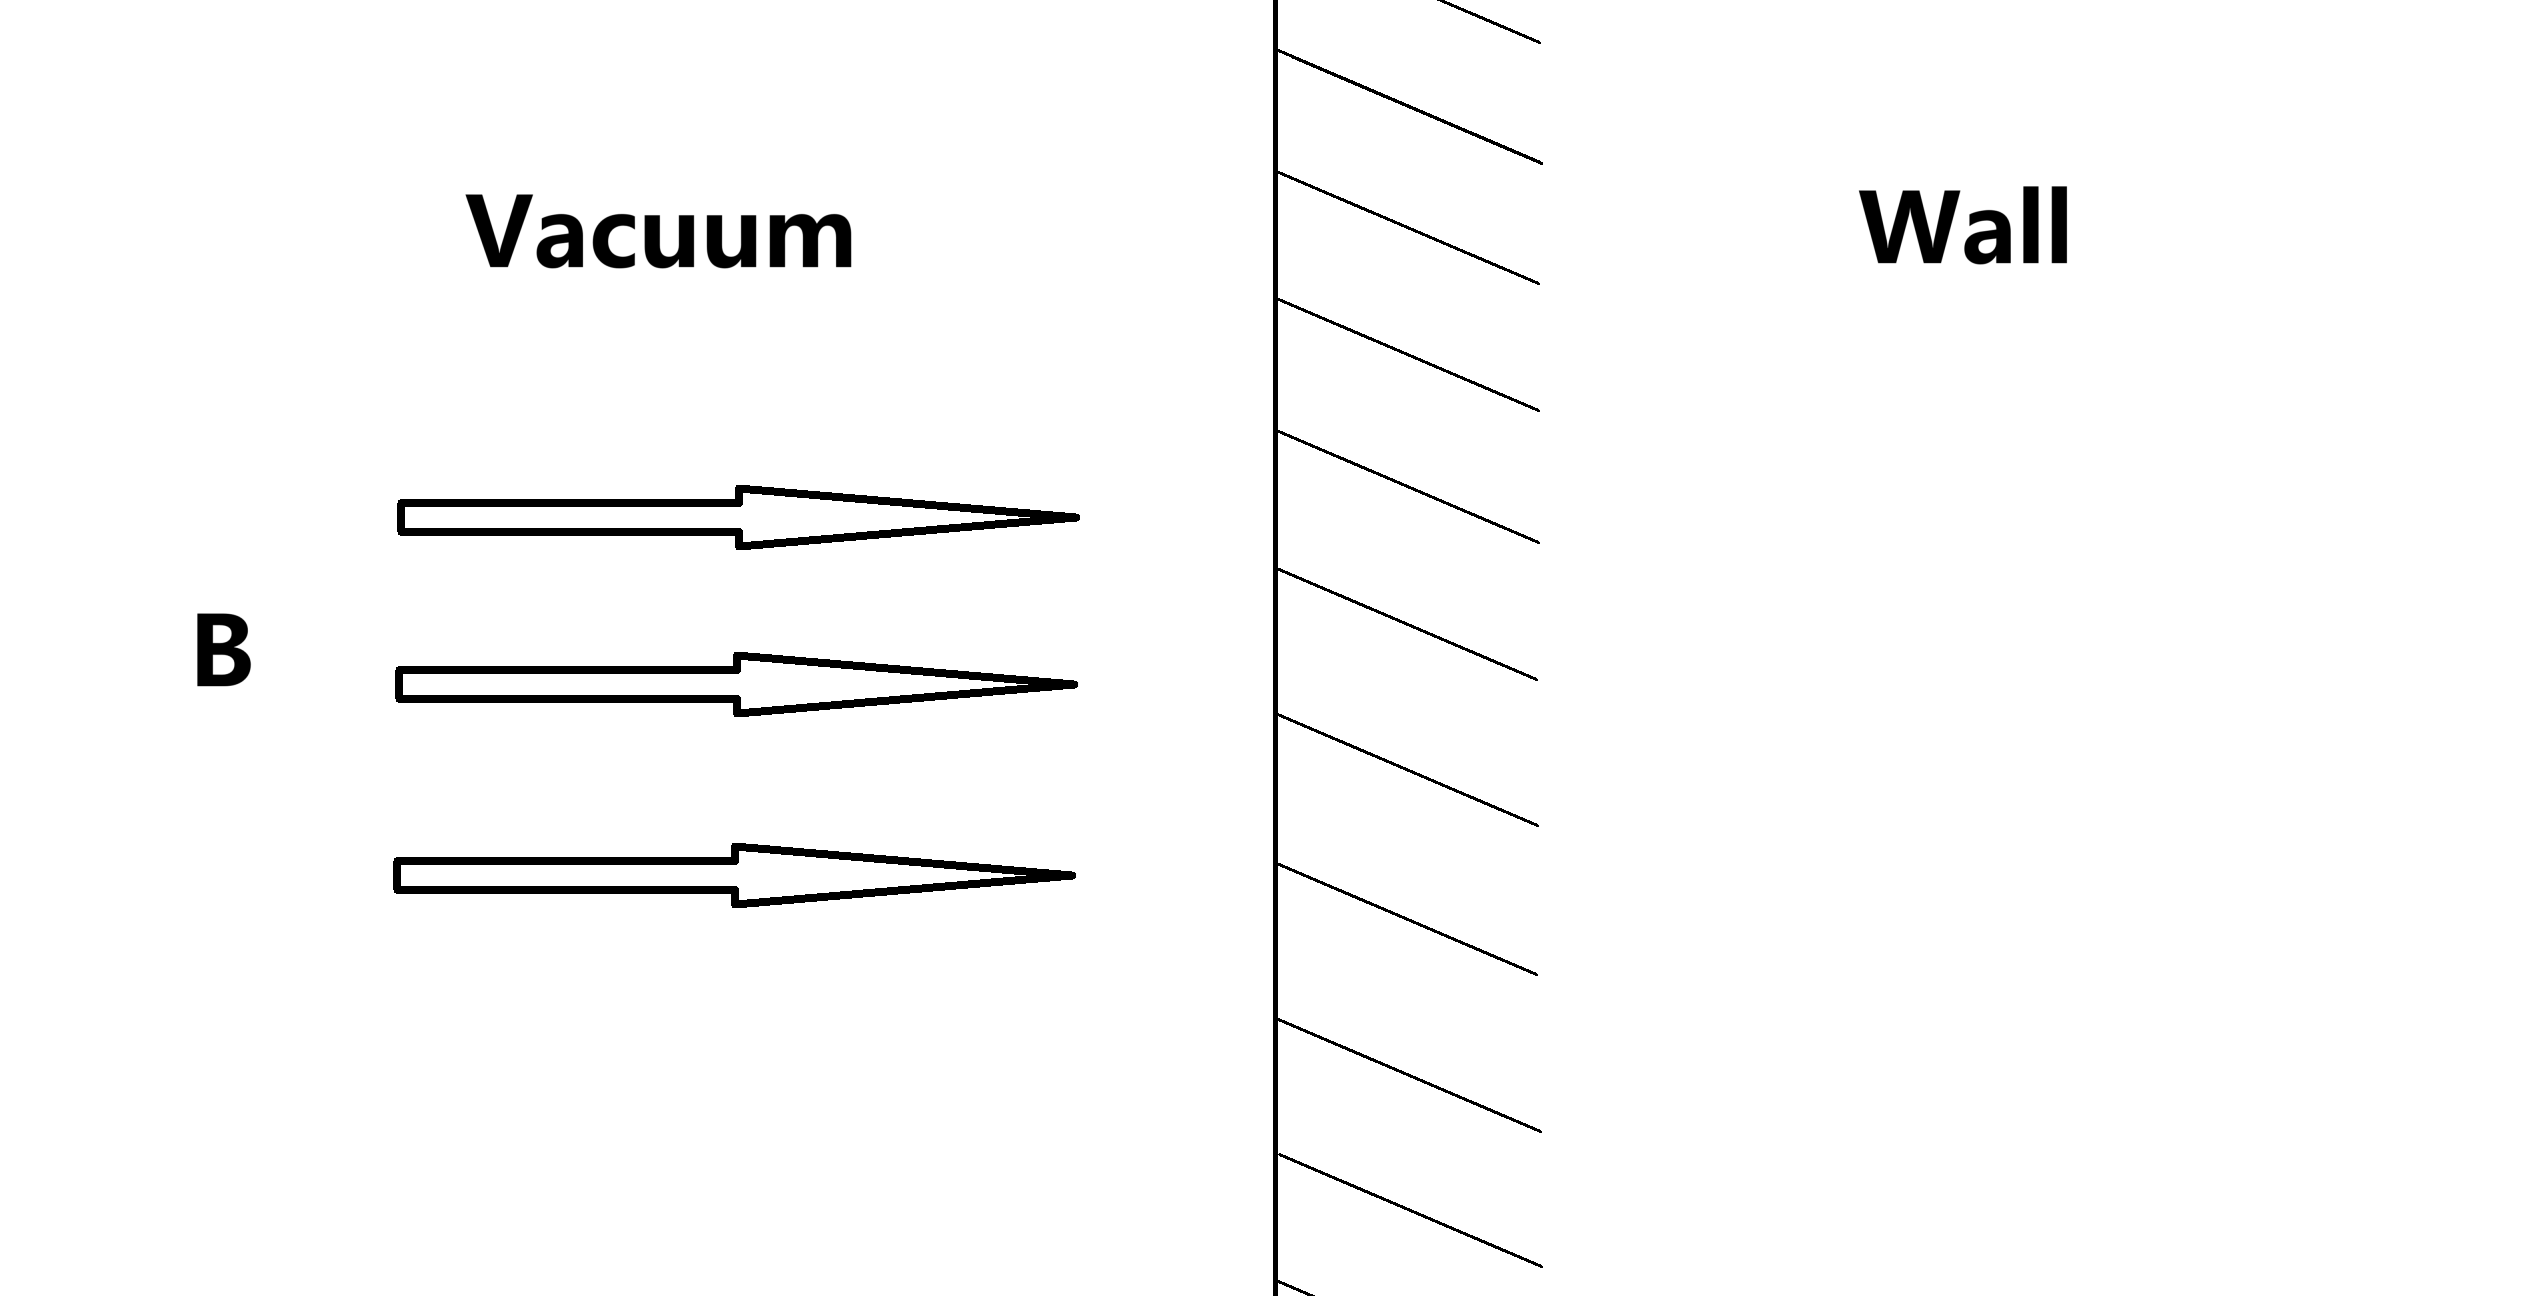
\includegraphics[width=0.8\linewidth]{BPenetration.png}
	\caption[Magnetic Penetration]{An illustration of normal magnetic field on a conducting wall. The entire space is divided into two parts: the left side ($x<0$) is a vacuum, and the right side ($x\geq0$) is a wall made of a certain conductor material. A homogeneous normal magnetic field $\mathbf{B}=B_0\mathbf{i}$ is suddenly imposed on the wall. The extent to which the magnetic field penetrates the wall depends on the resistivity of the wall's material.}
	\label{fig:magneticPenetration}
\end{figure}

\begin{figure}[H]
	\centering
	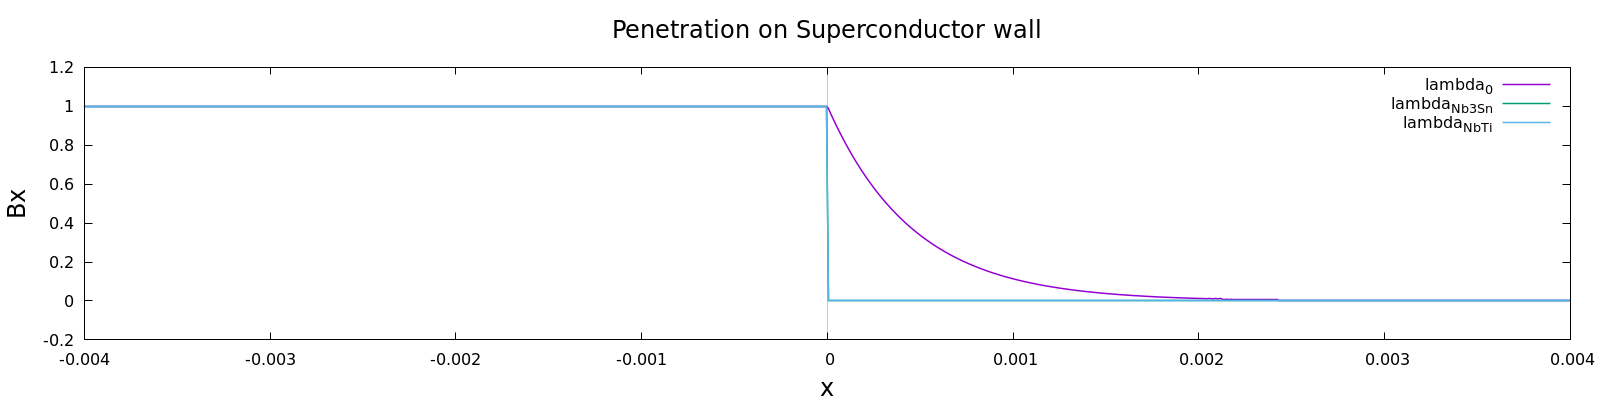
\includegraphics[width=1\linewidth]{penetration_superconducting.png}
	\caption[Bx Distribution]{Magnetic penetration along x for Nb3Sn and NbTi walls. For better visualization, nonphysical $\lambda_{0}=4.6\times10^{-4}m$ is add. The x-axis is scaled to 0.001 to keep a similar length with mesh refinement. It seems that once the magnetic field penetrates walls, it is fully countered off immediately in superconductors.}
	\label{fig:PenetrationCurveSuperconducting}
\end{figure}

\section{Extension on General Wall}
We make an extension into a general wall condition. A similar relationship still hold for current density based on free number density $n$,  
$$
\mathbf{J}=-n q_e \mathbf{v}\ .
$$
However, in Newton's Second Law of Motion, we need to consider the effect of resistivity. In microscopic point of view, electron collides when moving along conductor. We use collision frequency $\nu$ to represent such phenomenon. The resistivity $\eta_w$ and $\nu$ have relation $\eta_w=\frac{nq_e^2}{\nu m}$. In Kittle \cite{kittel2018introduction}, a similar collision time $\tau$ and conductivity are defined. From a macroscopic perspective, this behaves like damping \cite{kittel2018introduction}. The motion of an electron can be given by 
$$
m\frac{d\mathbf{v}}{dt}+m\nu \mathbf{v}=-q_eE\ .
$$

Solving this differential equation for $\mathbf{v}$ along with a initial condition $\mathbf{v}_0=0$, give the solution 
$$
\mathbf{v}=-\frac{q_e\mathbf{E}}{\nu m}+\frac{q_e\mathbf{E}}{\nu m}e^{-\nu t}\ .
$$

After taking curl and applying the Faraday's Law, some rearrangement is applied onto the equation. These give 
\begin{equation}
	\nabla^2\mathbf{B}=\frac{nq_e^2}{m\nu}\frac{\partial \mathbf{B}}{\partial t}-\frac{nq_e^2}{m\nu}e^{-\nu t}\frac{\partial \mathbf{B}}{\partial t}
	\label{equ:consistent_resistivewall}
\end{equation}

\section{Boundary Condition Recap} 
In this section, we show that the resistive wall equation \ref{equ:consistent_resistivewall} gives a more consistent boundary condition in the limit $\eta_{w}\to0$ with several boundary situations.
\subsection*{Perfect Conducting Wall}
For perfect conducting wall, L'Hopital's Rule gives $$
\lim_{\nu \to 0}\frac{1-e^{-\nu t}}{\nu}=\frac{\frac{\partial(1-e^{-\nu t})}{\partial \nu}}{\frac{\partial\nu}{\partial \nu}}=t\ .
$$ 
To eliminate a possible pre-existing magnetic field mathematically, perturbation methods may have applied. Assume that the change over time $\frac{\partial \mathbf{B}}{\partial t}$ is small. Maclaurin series for $\mathbf{B}$ give a linear approximation $t\frac{\partial \mathbf{B}}{\partial t}\approx\mathbf{B}$. It gives 
$$
\nabla^2\mathbf{B}=\frac{n q_e^2}{m}\mathbf{B}\ .
$$
This is the same as discussed in superconducting case. We have shown that a reflective Dirichlet boundary condition is appropriate in this case.

\subsection*{Resistive Wall and Insulator Wall}
For a resistive wall, $\nu$ is big enough and $e^{-\nu t}$ can be ignored. With relation $\eta_w=\frac{nq_e^2}{m\nu}$, we have 
$$
\eta_{w}\nabla^2\mathbf{B}=\frac{\partial \mathbf{B}}{\partial t}\ .
$$
This scenario is precisely what we address with the resistive wall in equation \ref{equ:magneticDiffusion_rearrange}. We handle this boundary condition by updating it using a similar approach to the ghost fluid methods, as discussed in earlier chapters. An insulator wall can be considered as a limiting case of this situation, where any spatial differences are immediately propagated away. Rather than evolving this condition under significant stiffness, it is more practical to treat it as a Neumann boundary condition.

\subsection*{Small Resistivity}
In the Plot \ref{fig:totalEnergy}, the inconsistency occurs when 
$$
\lim_{\nu \to 0,\eta_w \to 0}\ Resistive\ Wall \neq Perfect\ Conducting\ Wall\ .
$$
This equation enables us to know more about the situation when resistivity get close to 0 but not 0. We have series expansion of $e^{-\nu t}=\sum_{n=0}^{\infty}\frac{(-1)^n}{n!}\nu^nt^n$ and $\frac{1 - e^{-\nu t}}{\nu} = t e^{-\nu t} + O(\nu t^2)$. With the assumption that magnetic field changes slightly over time and $\nu$ is small, $te^{-\nu t}\frac{\partial \mathbf{B}}{\partial t}\approx\mathbf{B}e^{-\nu t}$. These give the equation 
\begin{equation*}
	\nabla^2\mathbf{B}=\frac{e^{-\nu t}}{\lambda^2}\mathbf{B}\ ,\ \ \ \ \ \  \lambda^2=\frac{m}{n q_e^2}\ .
\end{equation*}
A solution on x coordinate is
\begin{equation}
	B_x(x)=B_0e^{-\frac{xe^{-\frac{\nu t}{2}}}{\lambda}}\ .
\end{equation}

Figure \ref{fig:smallResistivityWall} demonstrate some visualization of this solution. For simplicity, we use $\nu=1.0$ and $\lambda_{0}=4.6\times10^{-4}m$. It seems that when the normal magnetic component is imposed on the small resistive wall, it reacts like a perfect conducting wall as in a superconducting situation. The only effect of resistivity is to gradually allow the magnetic field to penetrate the wall over time. Based on the numerical methods we have, the use of a reflective boundary condition for the plasma, combined with updates to the rigid body magnetic field, appears to offer a more accurate approximation for the boundary case characterized by low resistivity. However, due to the limited time available for this report, we were unable to conduct a comparative test of this method.  

\begin{figure}[H]
	\centering
	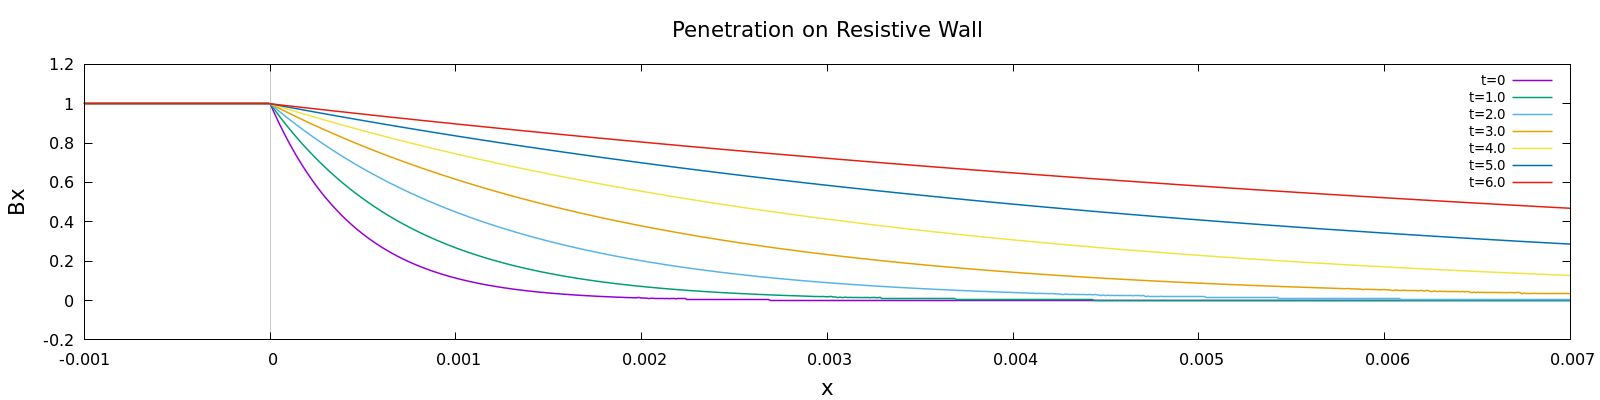
\includegraphics[width=1\linewidth]{penetration_wall.png}
	\caption[Bx Distribution on resistive wall]{Magnetic distribution on a resistive wall. When a normal magnetic field is applied to a small resistive wall, the initial magnetic field distribution inside behaves as if it were in a perfect conductor. However, the resistivity causes the magnetic field to slowly penetrate the wall over time.}
	\label{fig:smallResistivityWall}
\end{figure}
\section{Addressing the Inconsistency}
Generally, the inconsistency occurs when $\lim_{\eta_w \to 0}$. This is because we only consider a damping effect on electrons when $\eta_w>0$ in Maxwell's equation of $\eta_w\mathbf{J}=\mathbf{E}$ at a macroscopic level. However, for $\eta_w=0$, acceleration is the only factor considered. For example, in London Equations $m\frac{d\mathbf{v}_s}{dt}=-q_e\mathbf{E}$, where the electric field accelerates electrons infinitely. Hence, inconsistency occurs when neither of these effects can dominate, $\lim_{\eta_w \to 0}$. In such case, considering both effects may help on improving the consistency. There may be methods addressing this inconsistency considering both by compromising Neumann and Dirichlet condition, such as the Robin boundary condition proposed by Strauss \cite{strauss2014velocity}. Equation \ref{equ:consistent_resistivewall} and a similar plot to Figure \ref{fig:smallResistivityWall} will provide a strong reference for calculating the combination ratio in the Robin condition. Nevertheless, due to time constraints, this approach was not implemented in report 2. Further research could explore this in more detail.